\documentclass[svgnames]{beamer}
\usetheme{Dresden}
\usecolortheme{beaver}
\usepackage{textcomp}
\usepackage{color}
\usepackage{colortbl}
\usepackage{pbox}
\setbeamerfont{page number in head/foot}{size=\large}
\setbeamertemplate{footline}[frame number]
\title{An experimental study of the learnability of congestion control}
\author{Anirudh~Sivaraman, Keith~Winstein, Pratiksha~Thaker, Hari~Balakrishnan}
\institute{MIT CSAIL\vspace{\baselineskip}\\\textcolor{DarkBlue}{http://web.mit.edu/remy/learnability}
}
%\\\textcolor{DarkBlue}{http://web.mit.edu/anirudh/www/sdn-data-plane.html}}
%\date{}
\definecolor{darkgreen}{rgb}{0.0, 0.2, 0.13}

\begin{document}

\begin{frame}

\titlepage

\end{frame}

\begin{Large}
%%%\begin{frame}
%%%\frametitle{Congestion-control protocols today}
%%%\begin{itemize}
%%%\item<2-> Implicit assumptions
%%%\item<3-> Implicit performance goals
%%%\end{itemize}
%%%\end{frame}
%%%
%%%\begin{frame}
%%%\frametitle{But, assumptions eventually don't hold}
%%%\begin{itemize}
%%%\item<2-> Links become much faster (transatlantic cables, datacenters)
%%%\item<3-> The number of senders increases (incast)
%%%%\item<3-> Delays get longer: satellite links
%%%\end{itemize}
%%%\end{frame}

\begin{frame}
\frametitle{This talk}
\begin{itemize}
\item<1->{How easy is it to “learn” a network protocol to achieve a desired goal,
despite a mismatched set of assumptions?}
\item<2->{cf. Learning: ``Knowledge acquisition without explicit programming'' (Valiant 1984)}
\end{itemize}
\end{frame}

%%\begin{frame}
%%\frametitle{Preview of key results}
%%\begin{itemize}
%%\item<2-> \textcolor{darkgreen}{Can tolerate mismatched link-rate assumptions}
%%\item<3-> \textcolor{red}{Need precision about the number of senders}
%%\item<4-> \textcolor{red}{TCP compatibility is a double-edged sword}
%%\item<5-> \textcolor{darkgreen}{Can tolerate mismatch in the \# of bottlenecks}
%%\end{itemize}
%%\end{frame}

\begin{frame}
\frametitle{Experimental method}
\noindent \only<2>{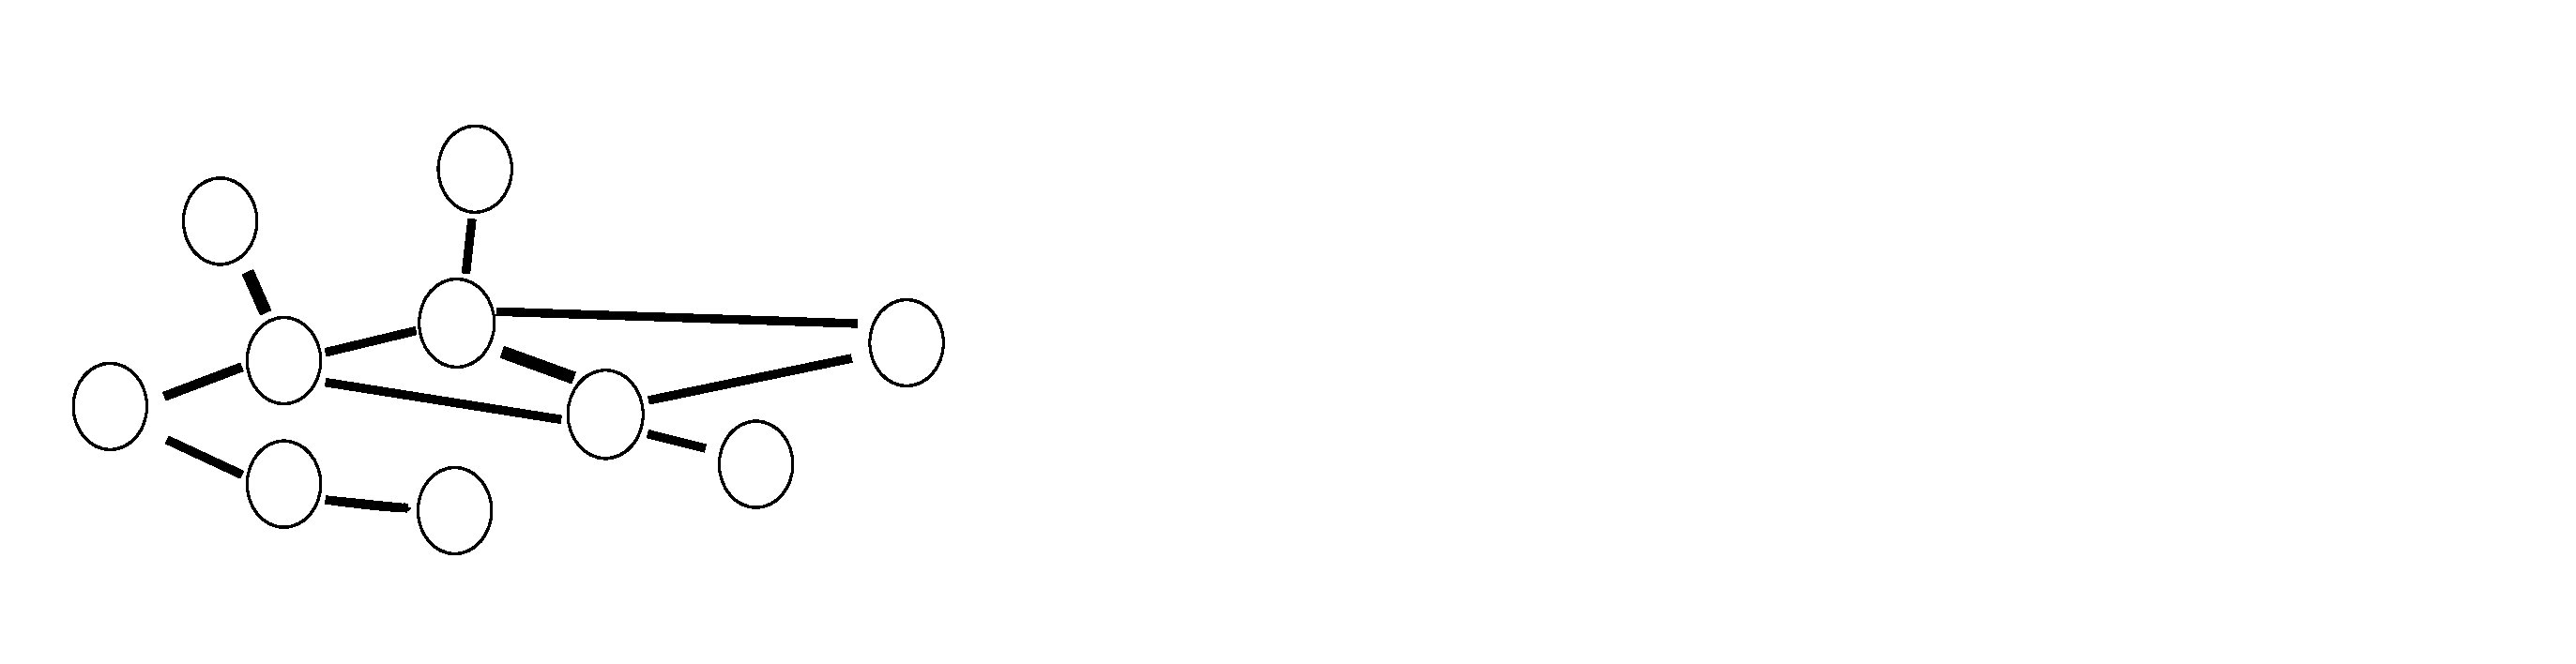
\includegraphics[width=5.5 in]{network-base.pdf}}\only<3>{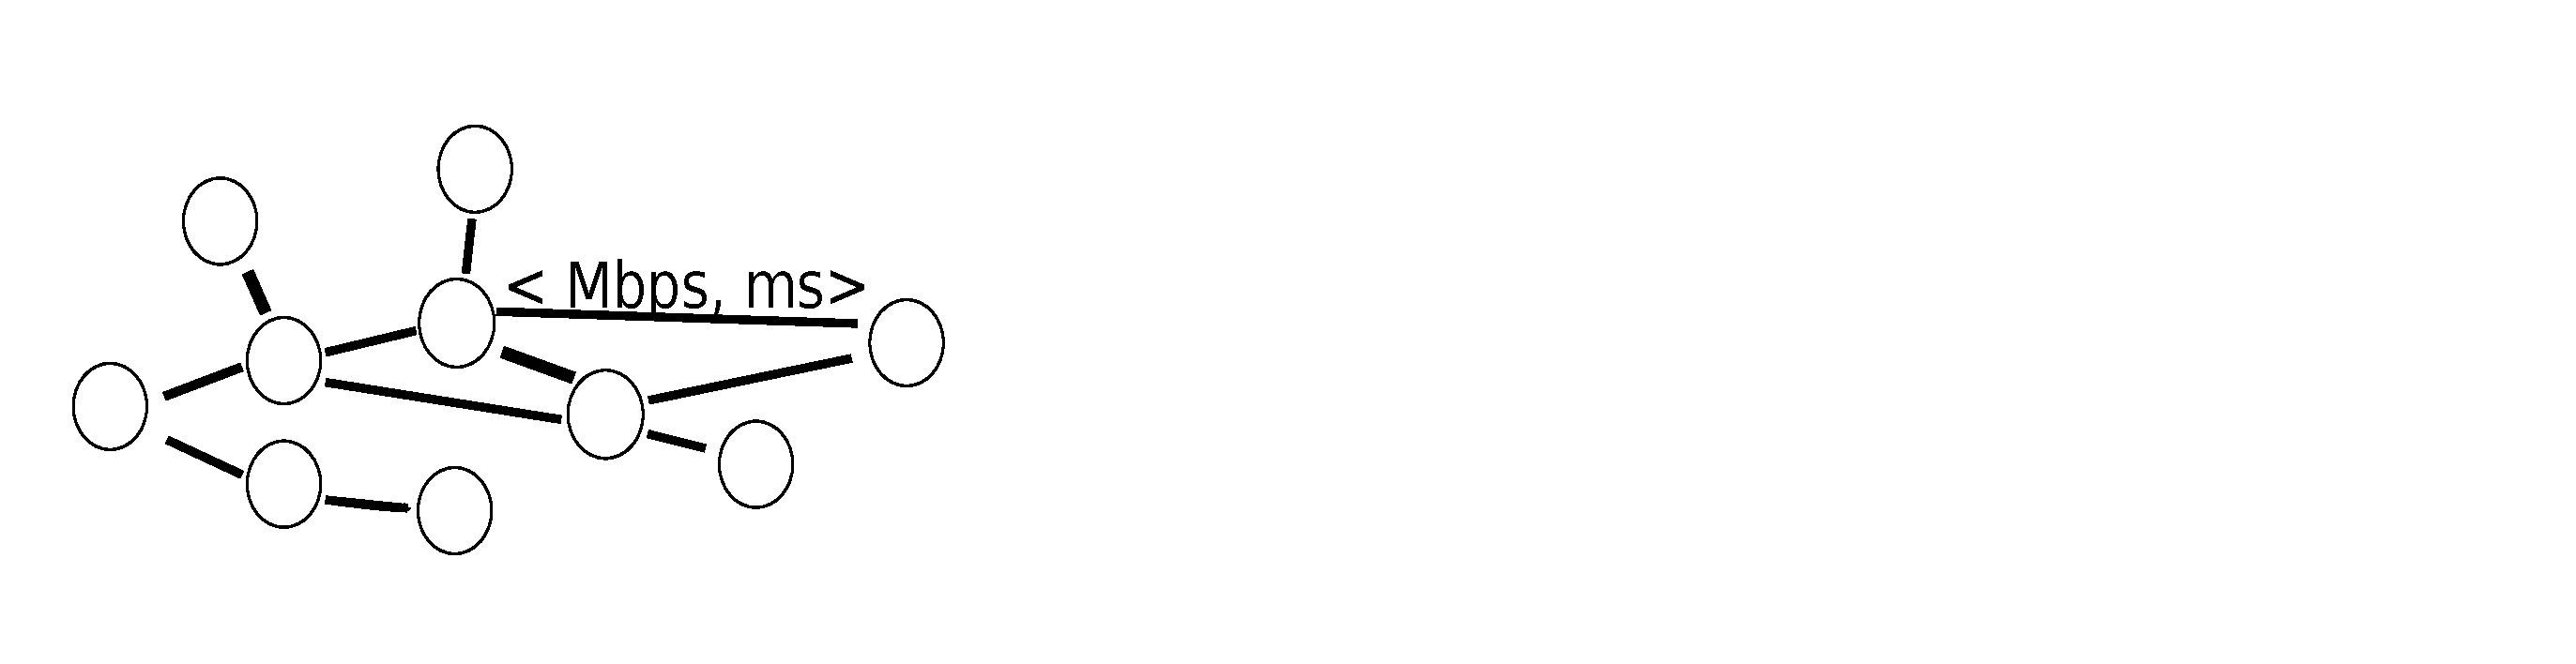
\includegraphics[width=5.5 in]{network-link.pdf}}\only<4>{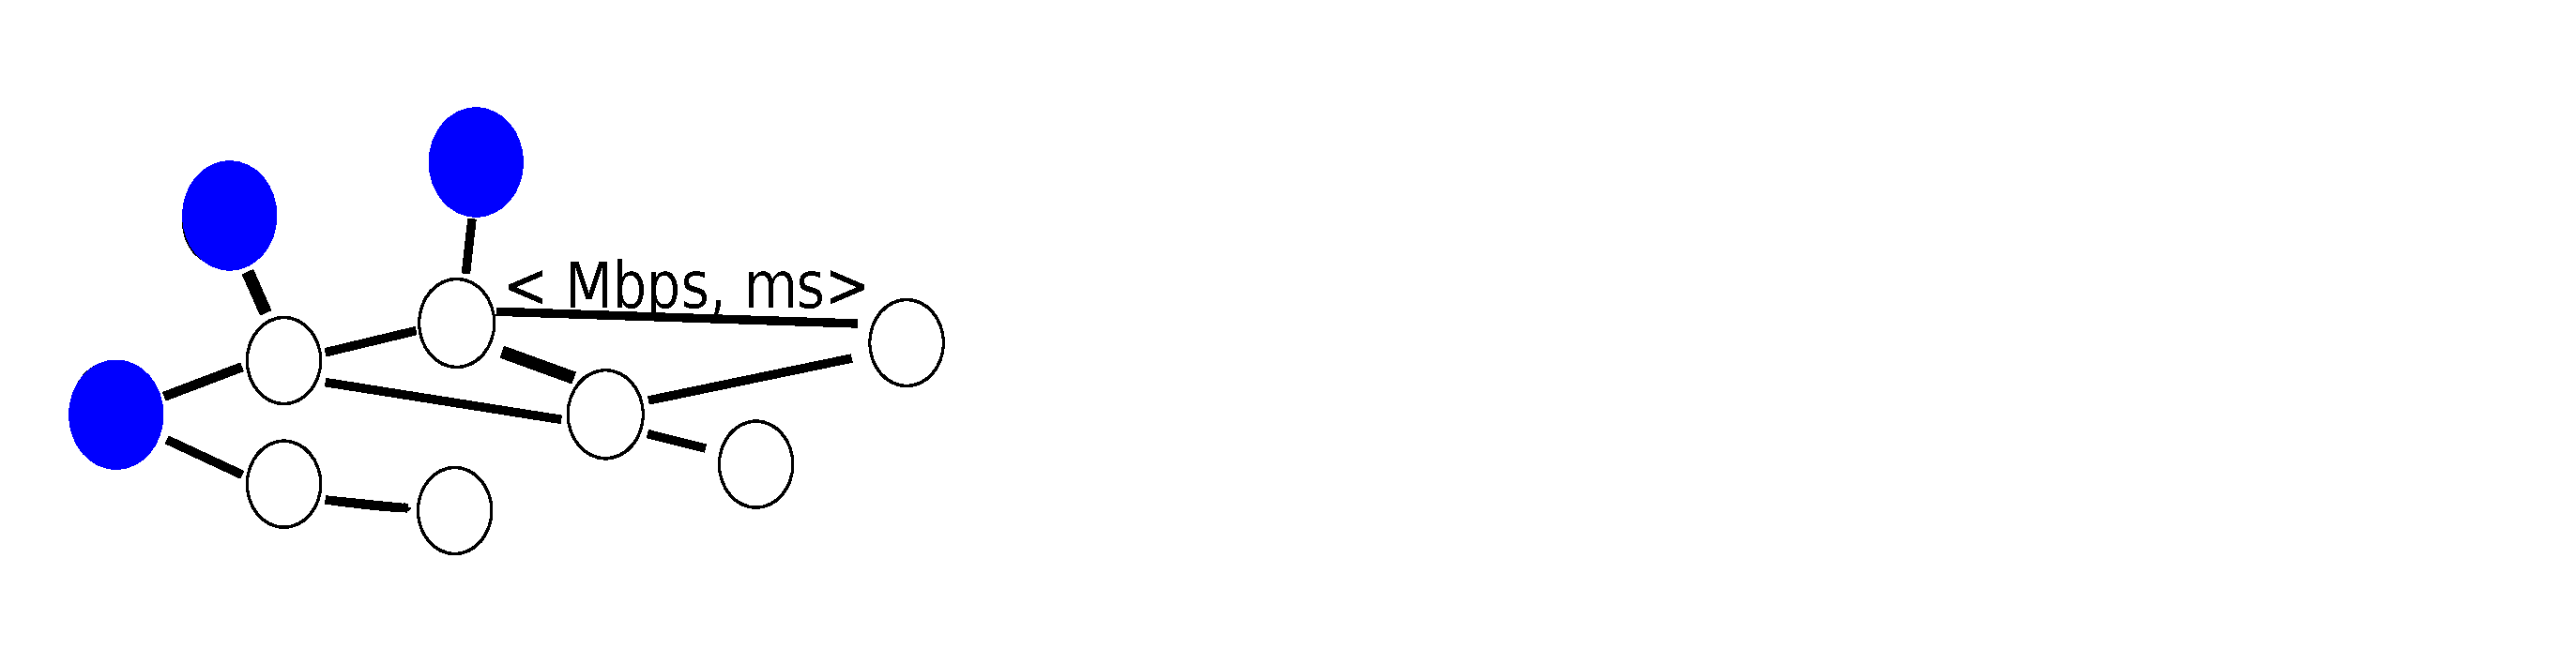
\includegraphics[width=5.5 in]{network-senders.pdf}}\only<5>{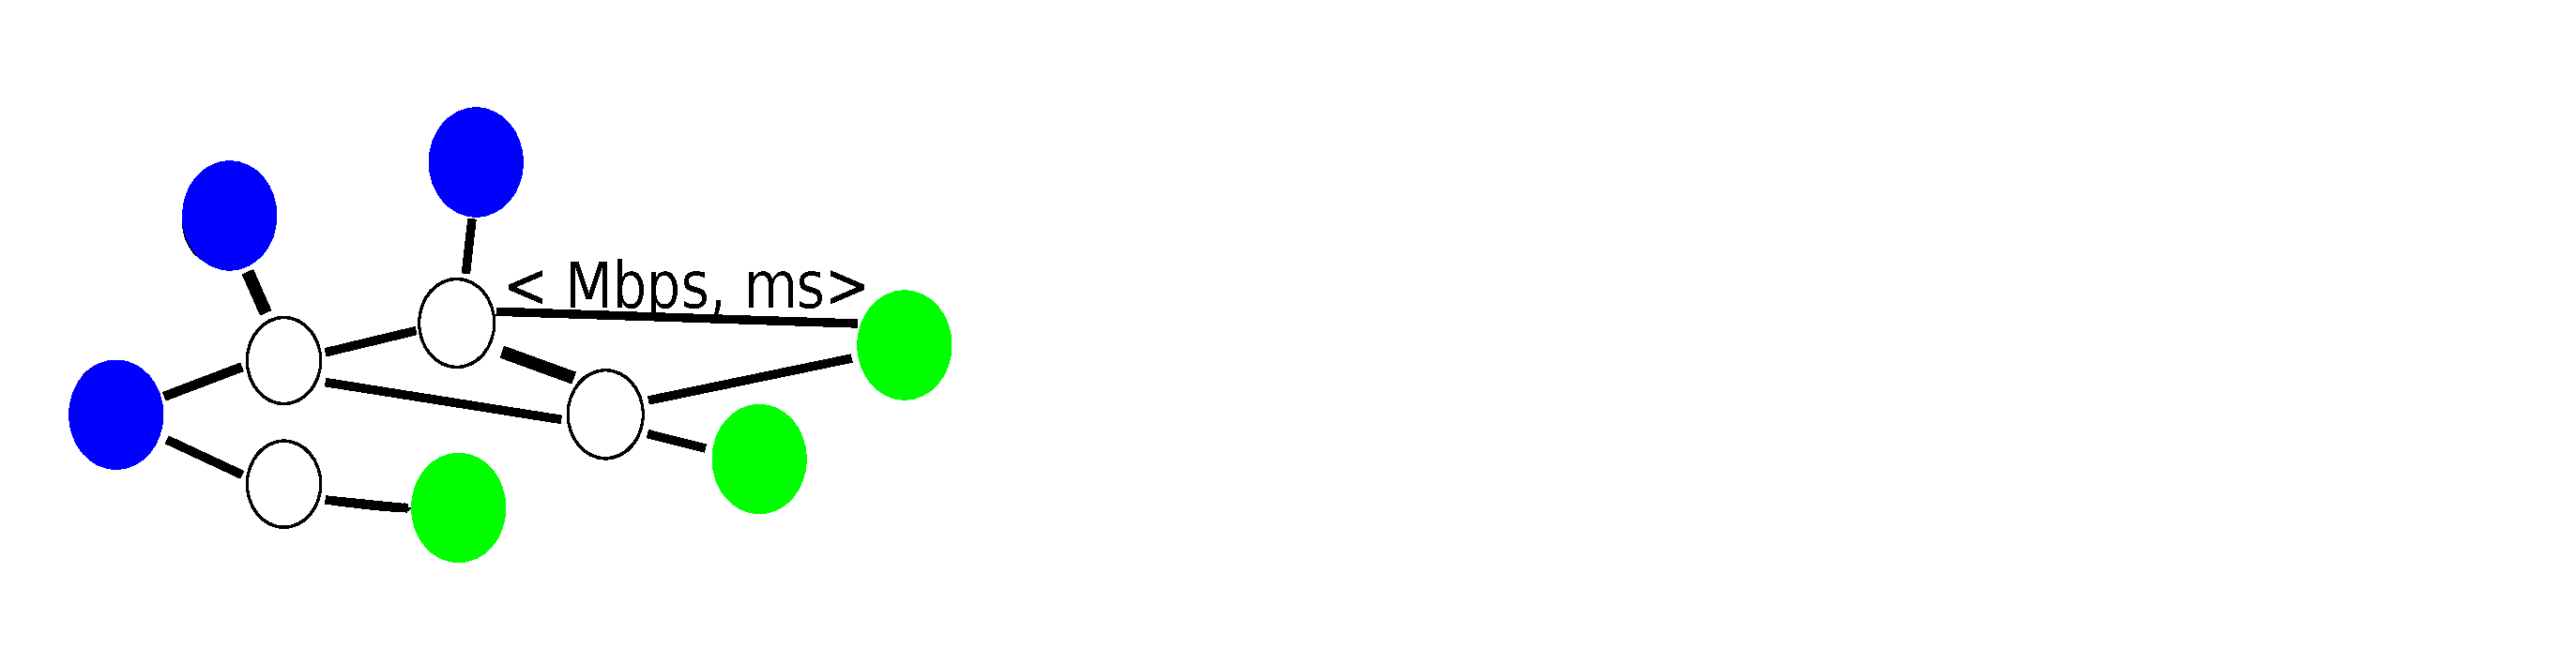
\includegraphics[width=5.5 in]{network-receivers.pdf}}\only<6>{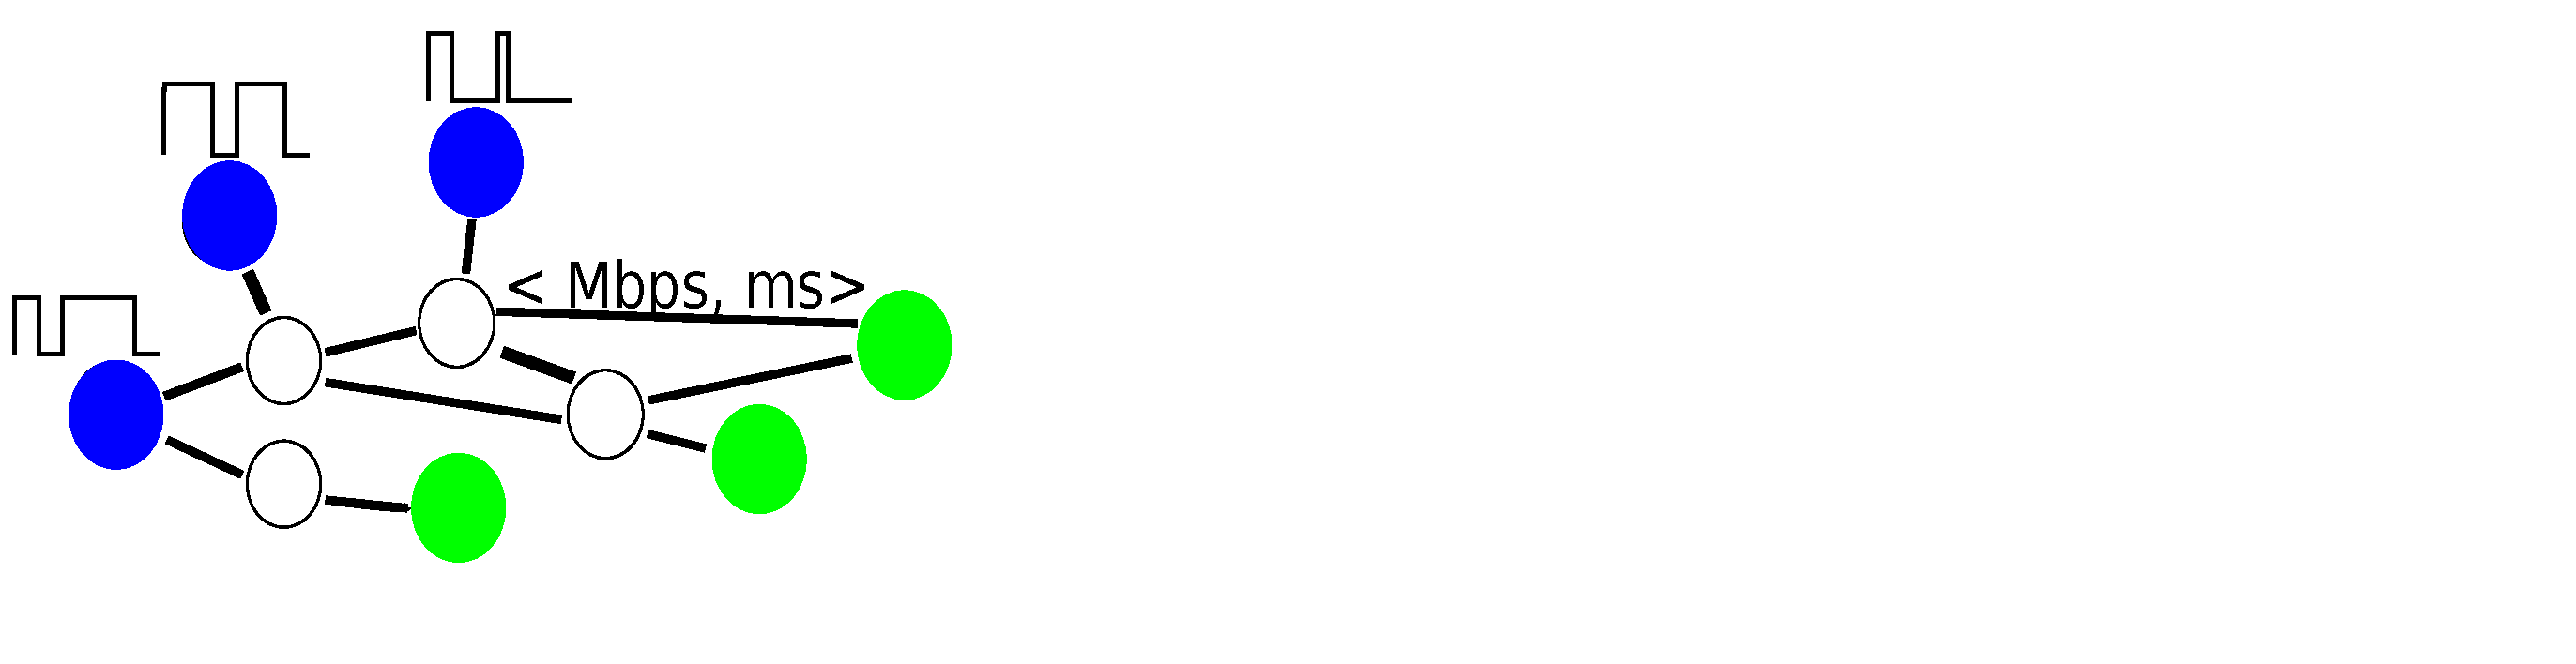
\includegraphics[width=5.5in]{network-application.pdf}}\only<7>{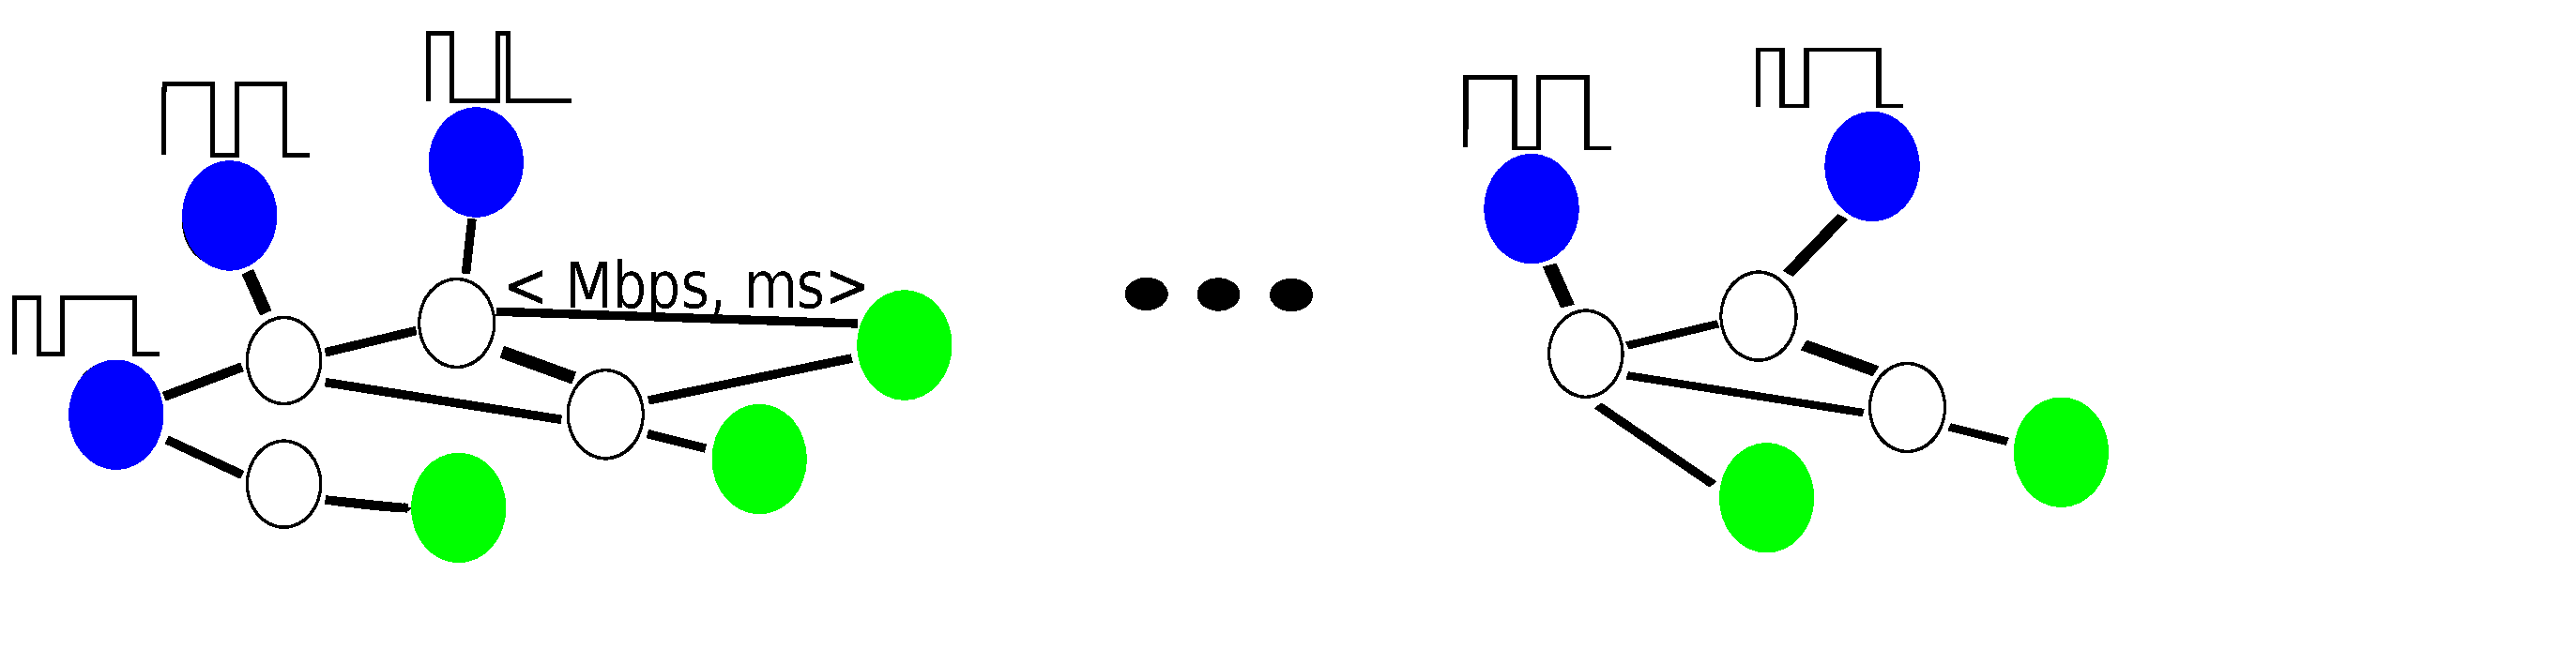
\includegraphics[width=5.5 in]{network-onemore.pdf}}
\end{frame}

\begin{frame}
\frametitle{Experimental method}
\noindent \only<1>{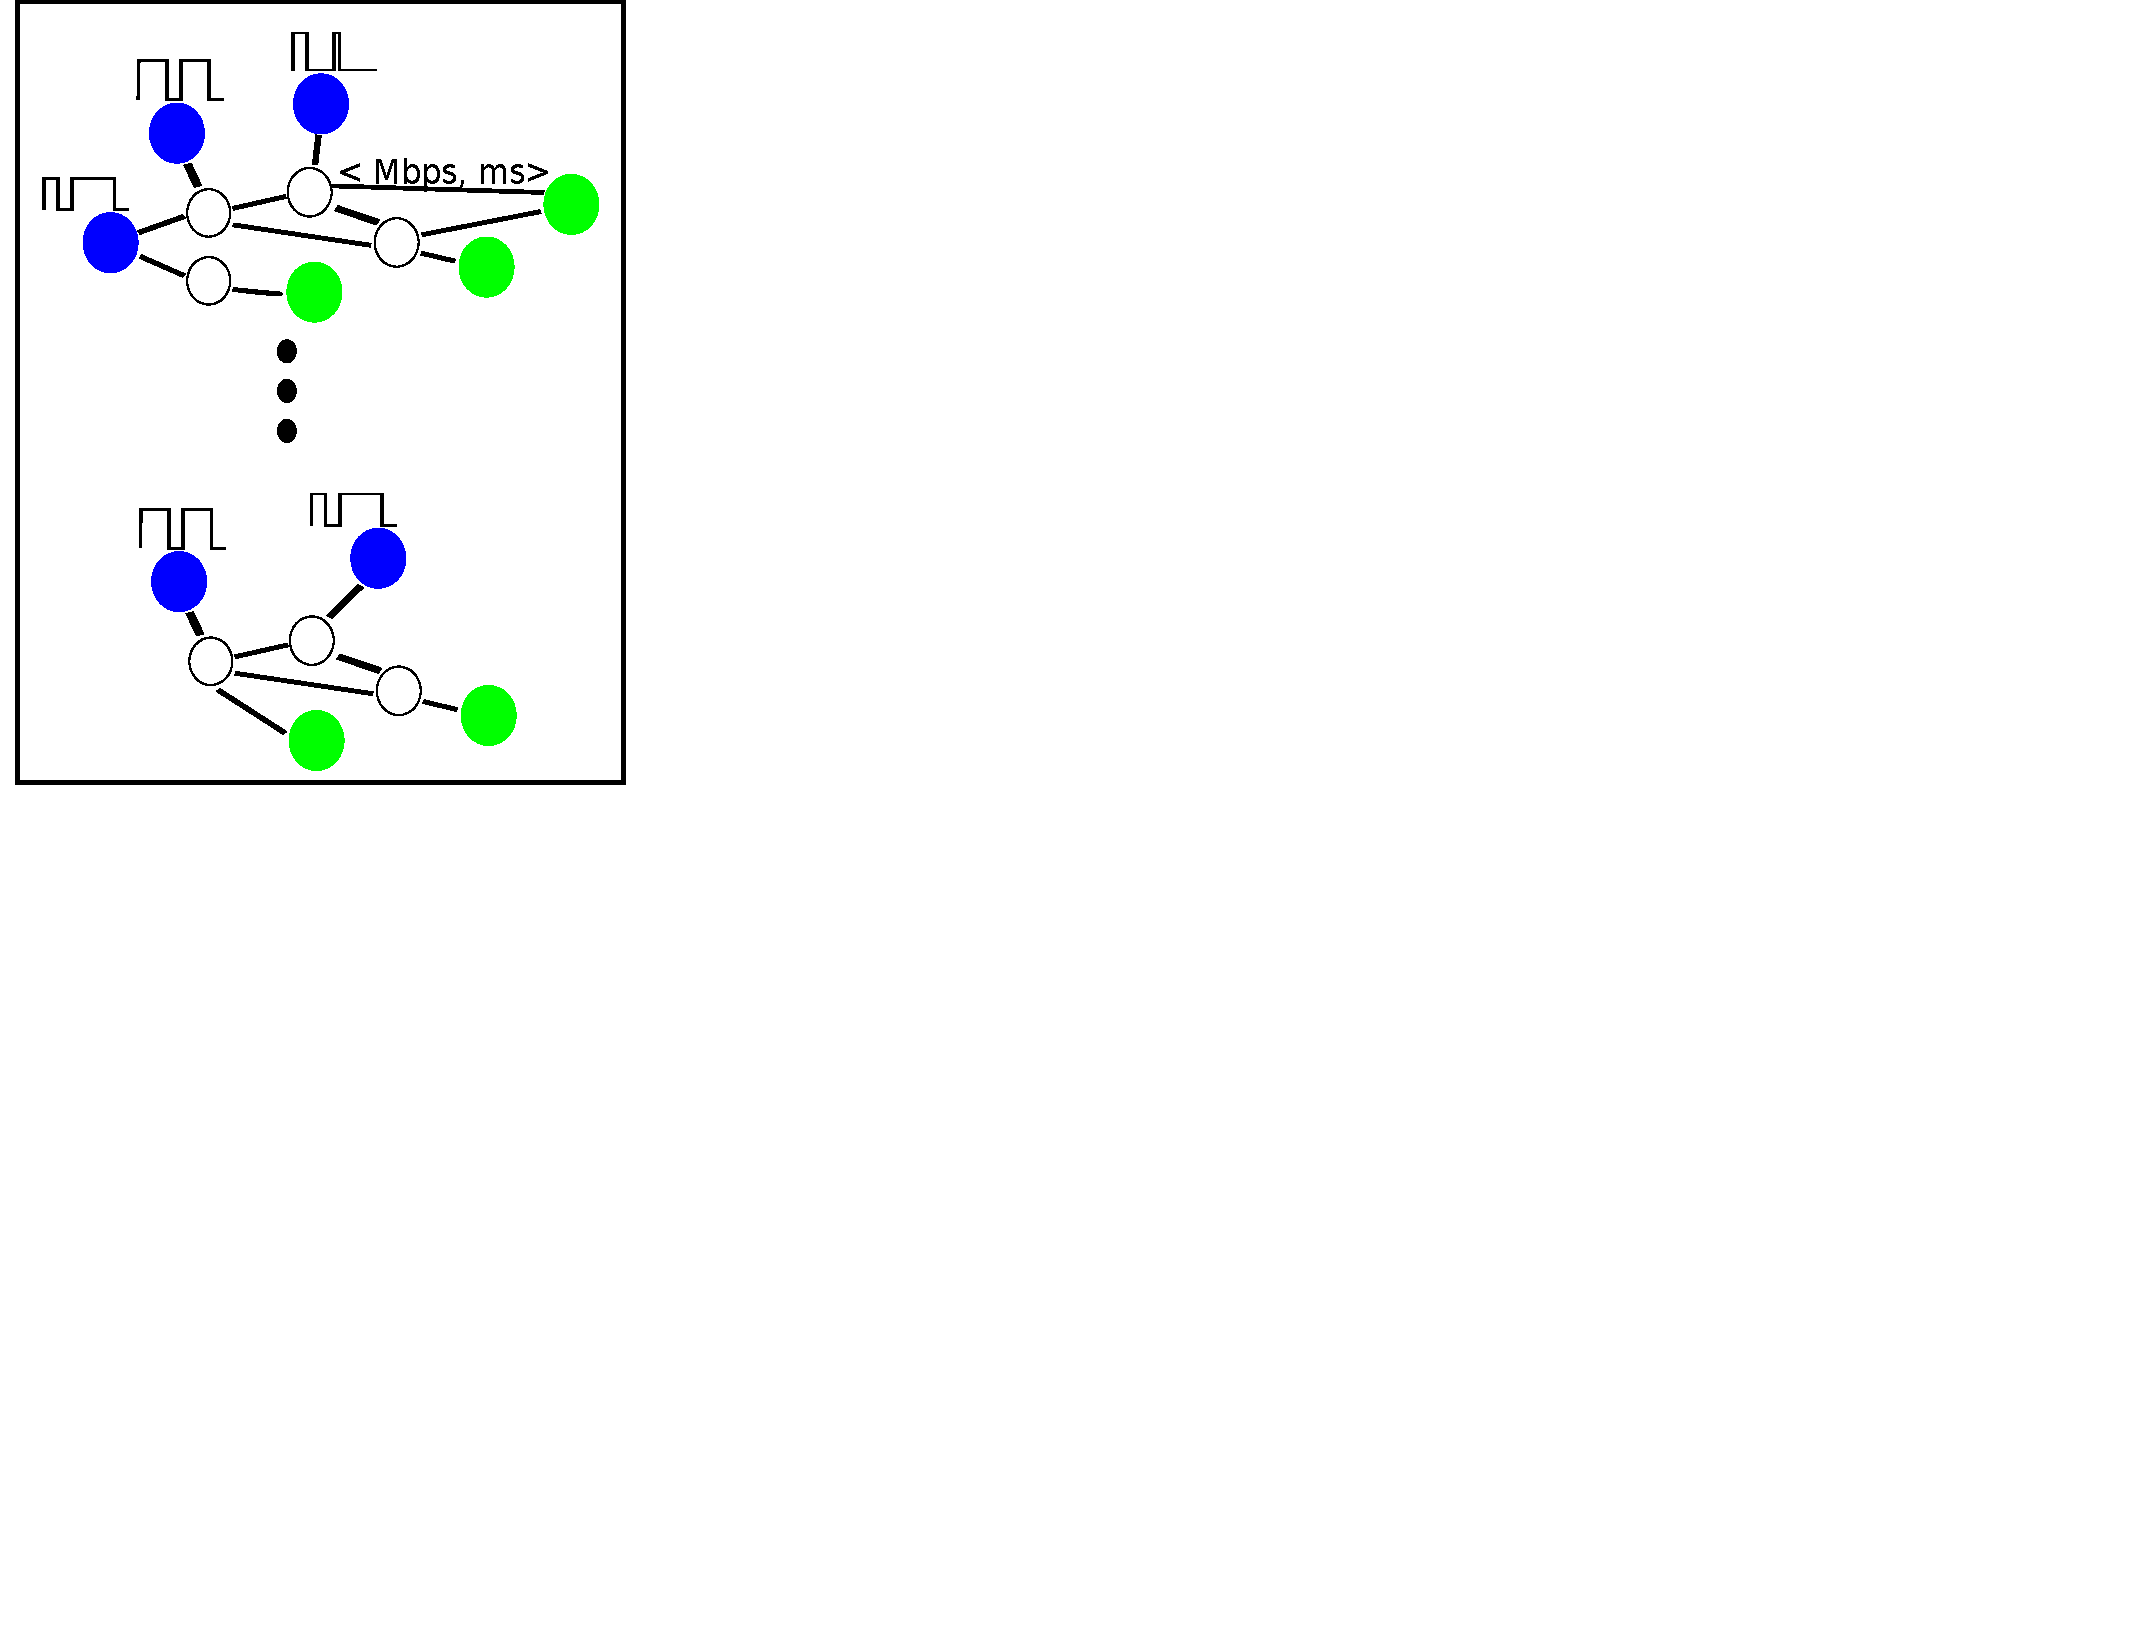
\includegraphics[width=4.5 in]{mechanize-1.pdf}}\only<2>{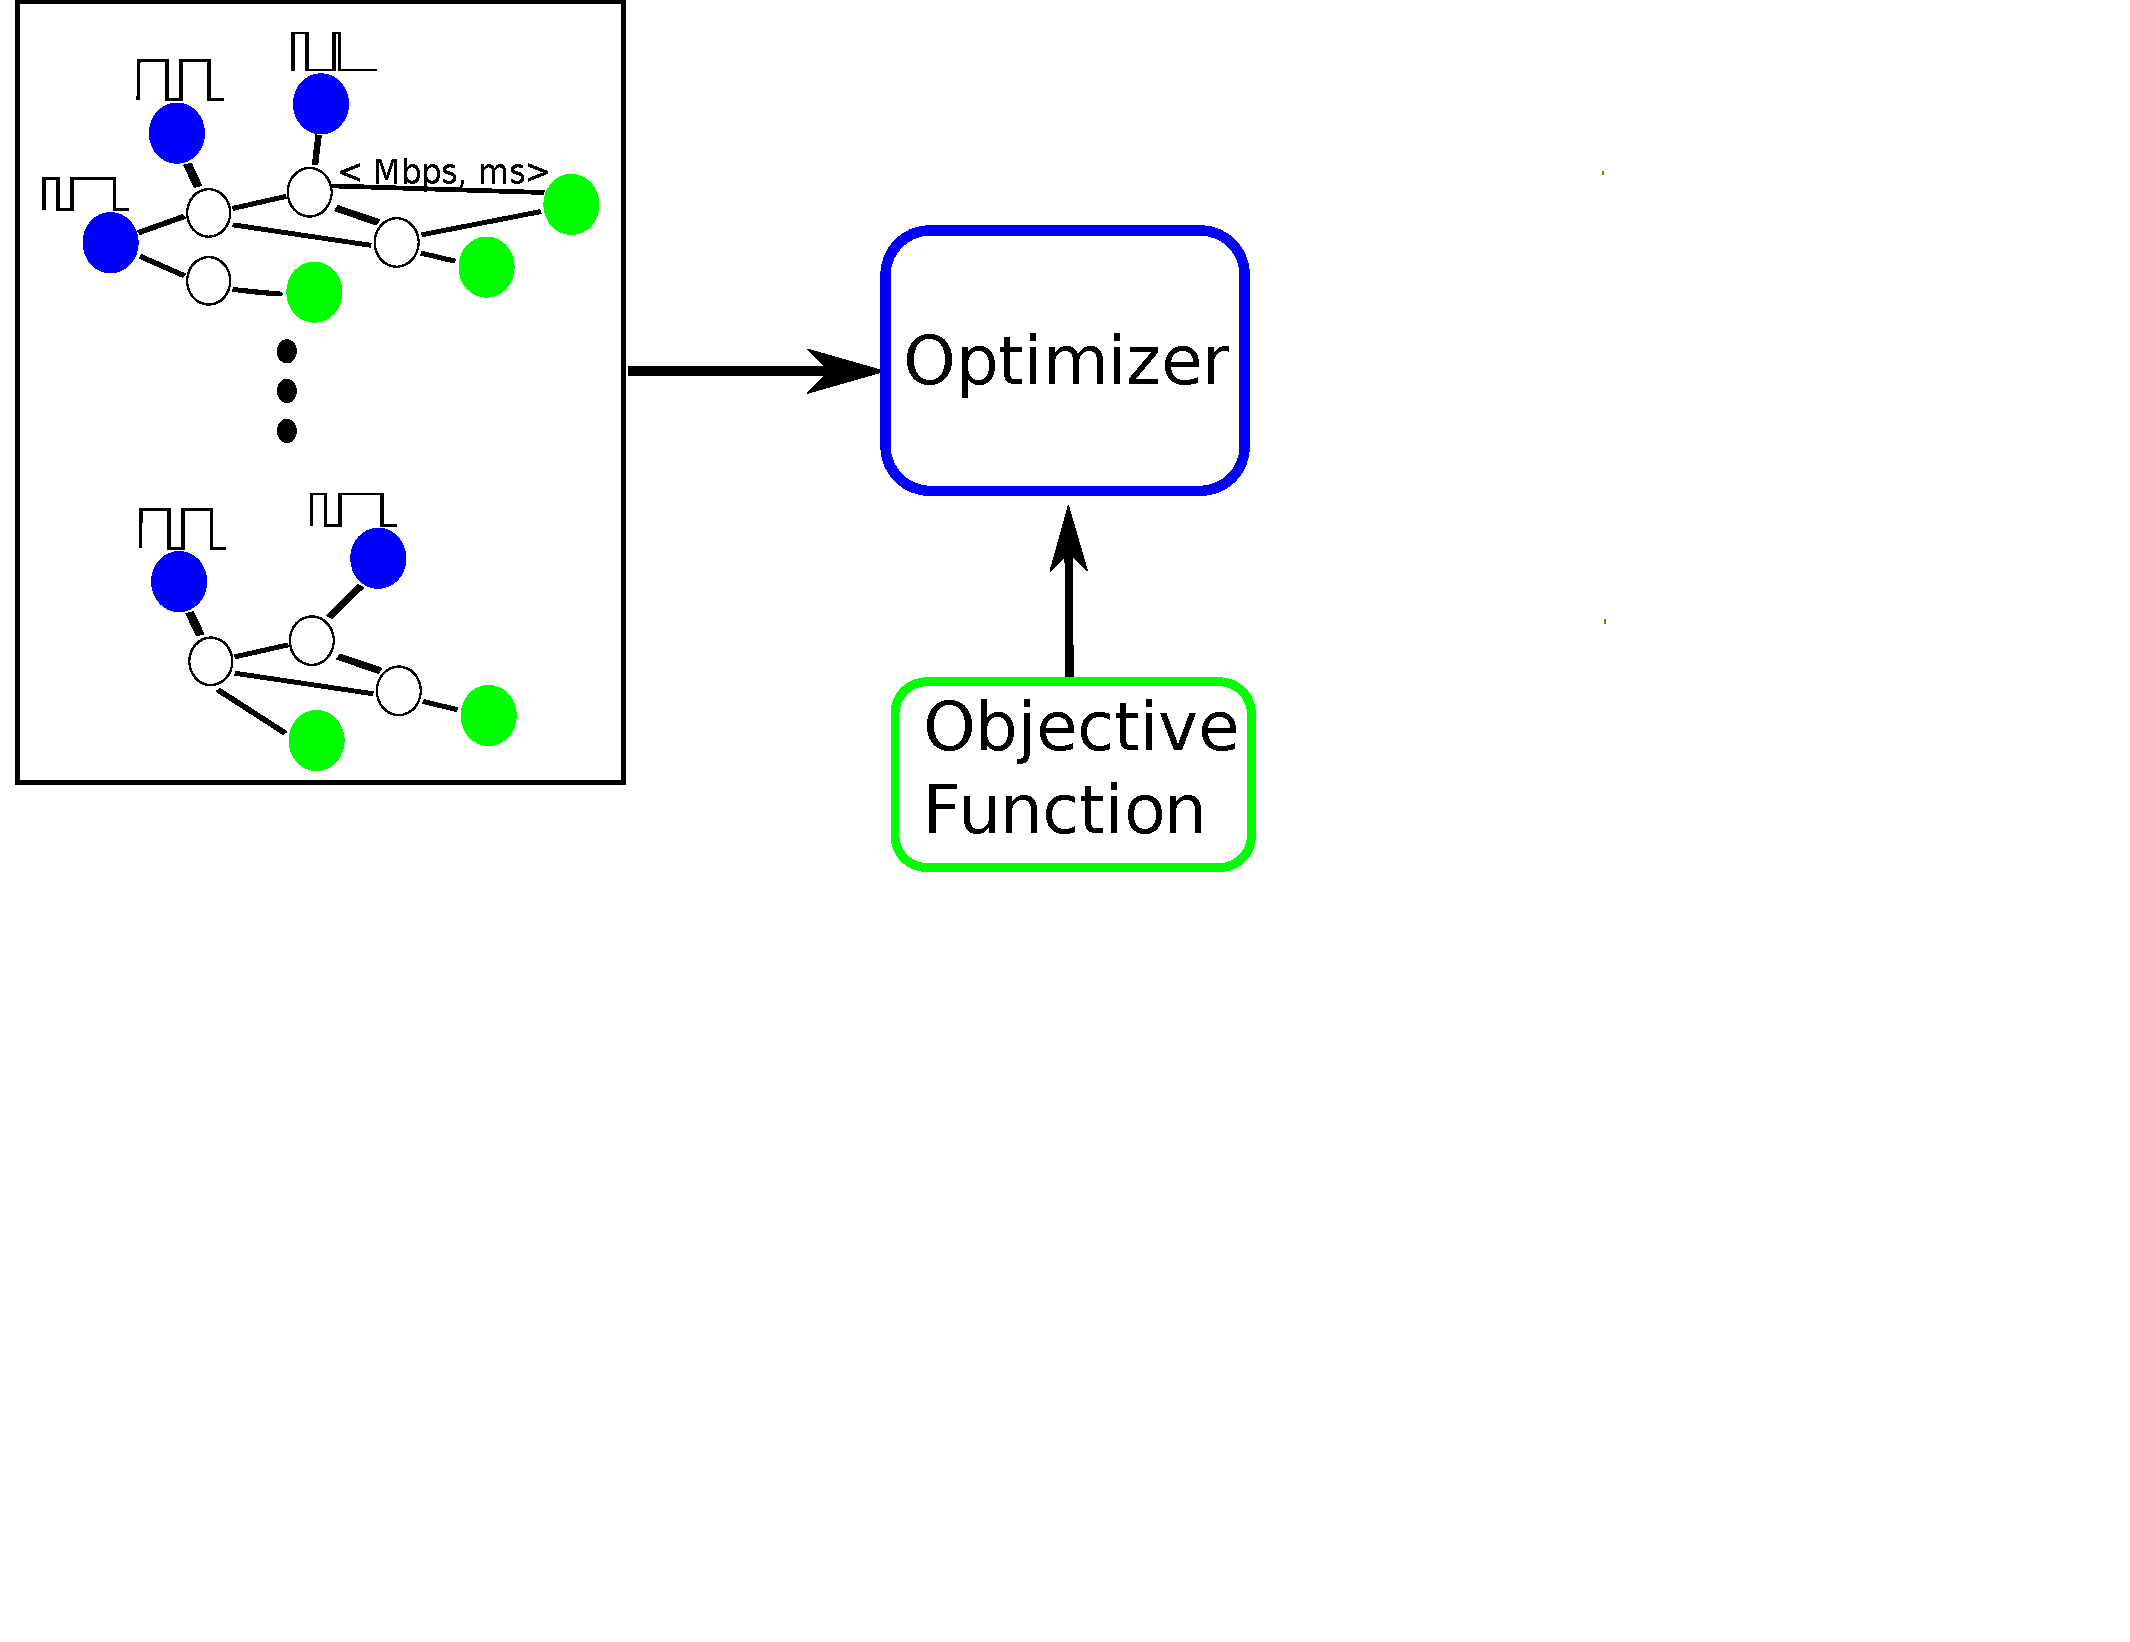
\includegraphics[width=4.5 in]{mechanize-2.pdf}}\only<3>{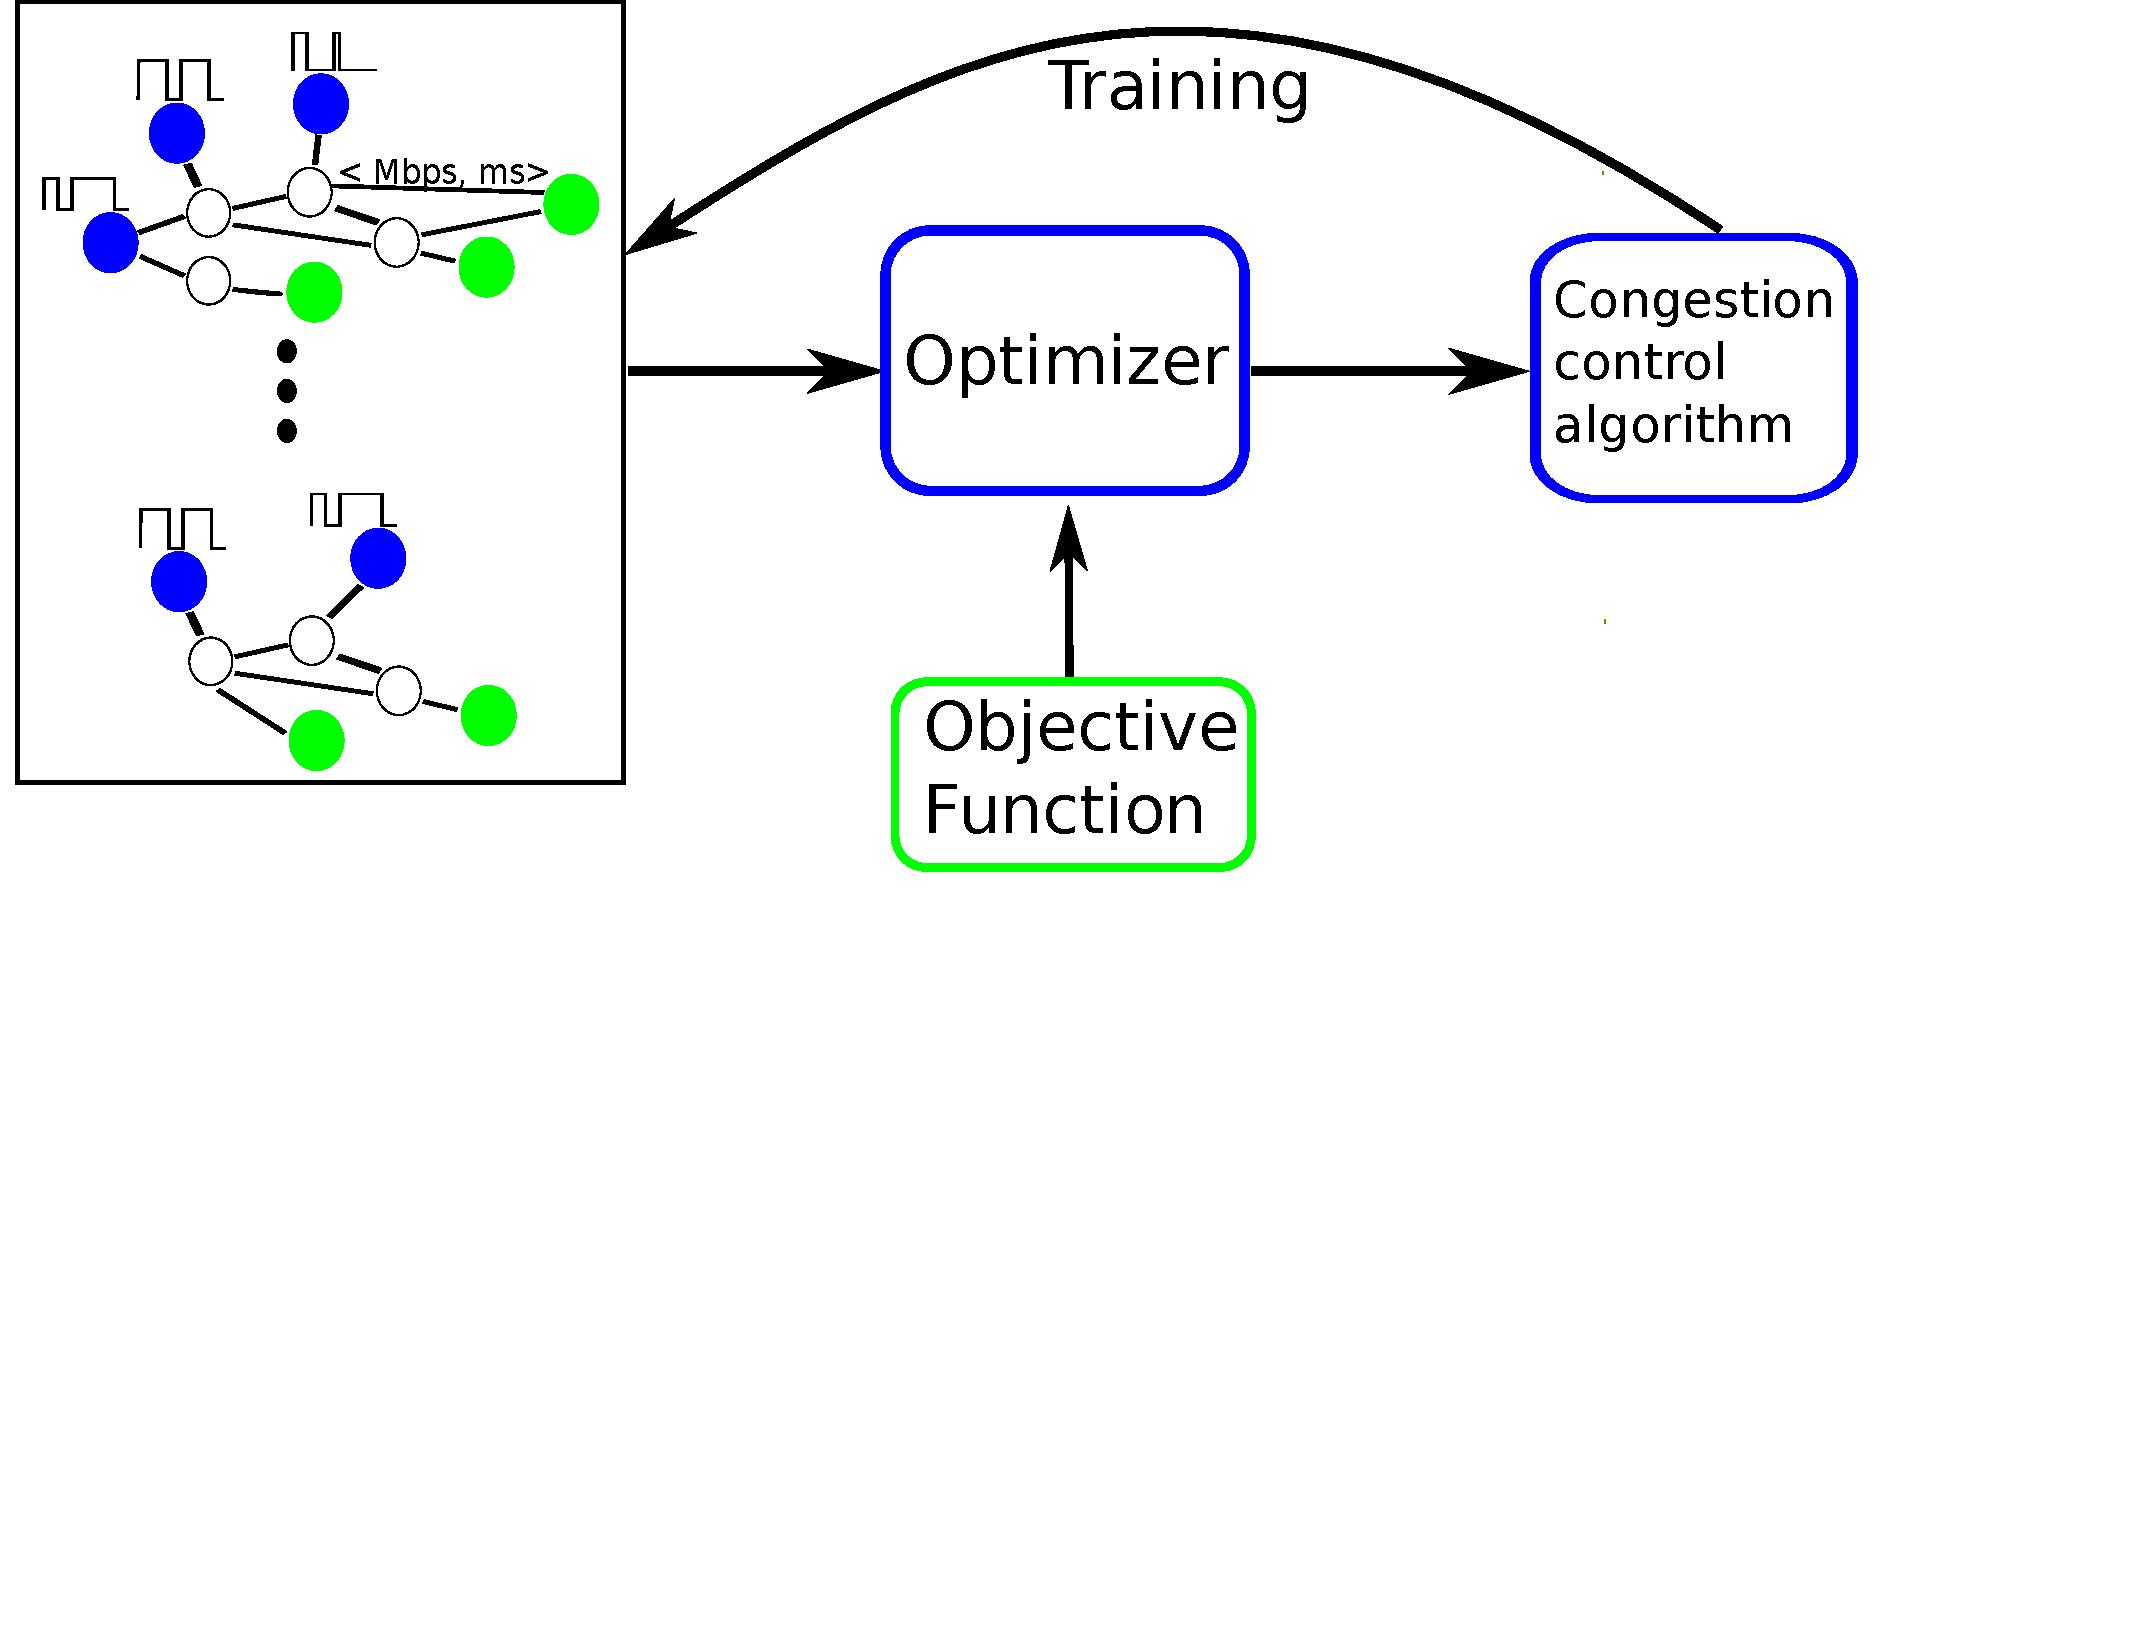
\includegraphics[width=4.5 in]{mechanize-3.pdf}}\only<4>{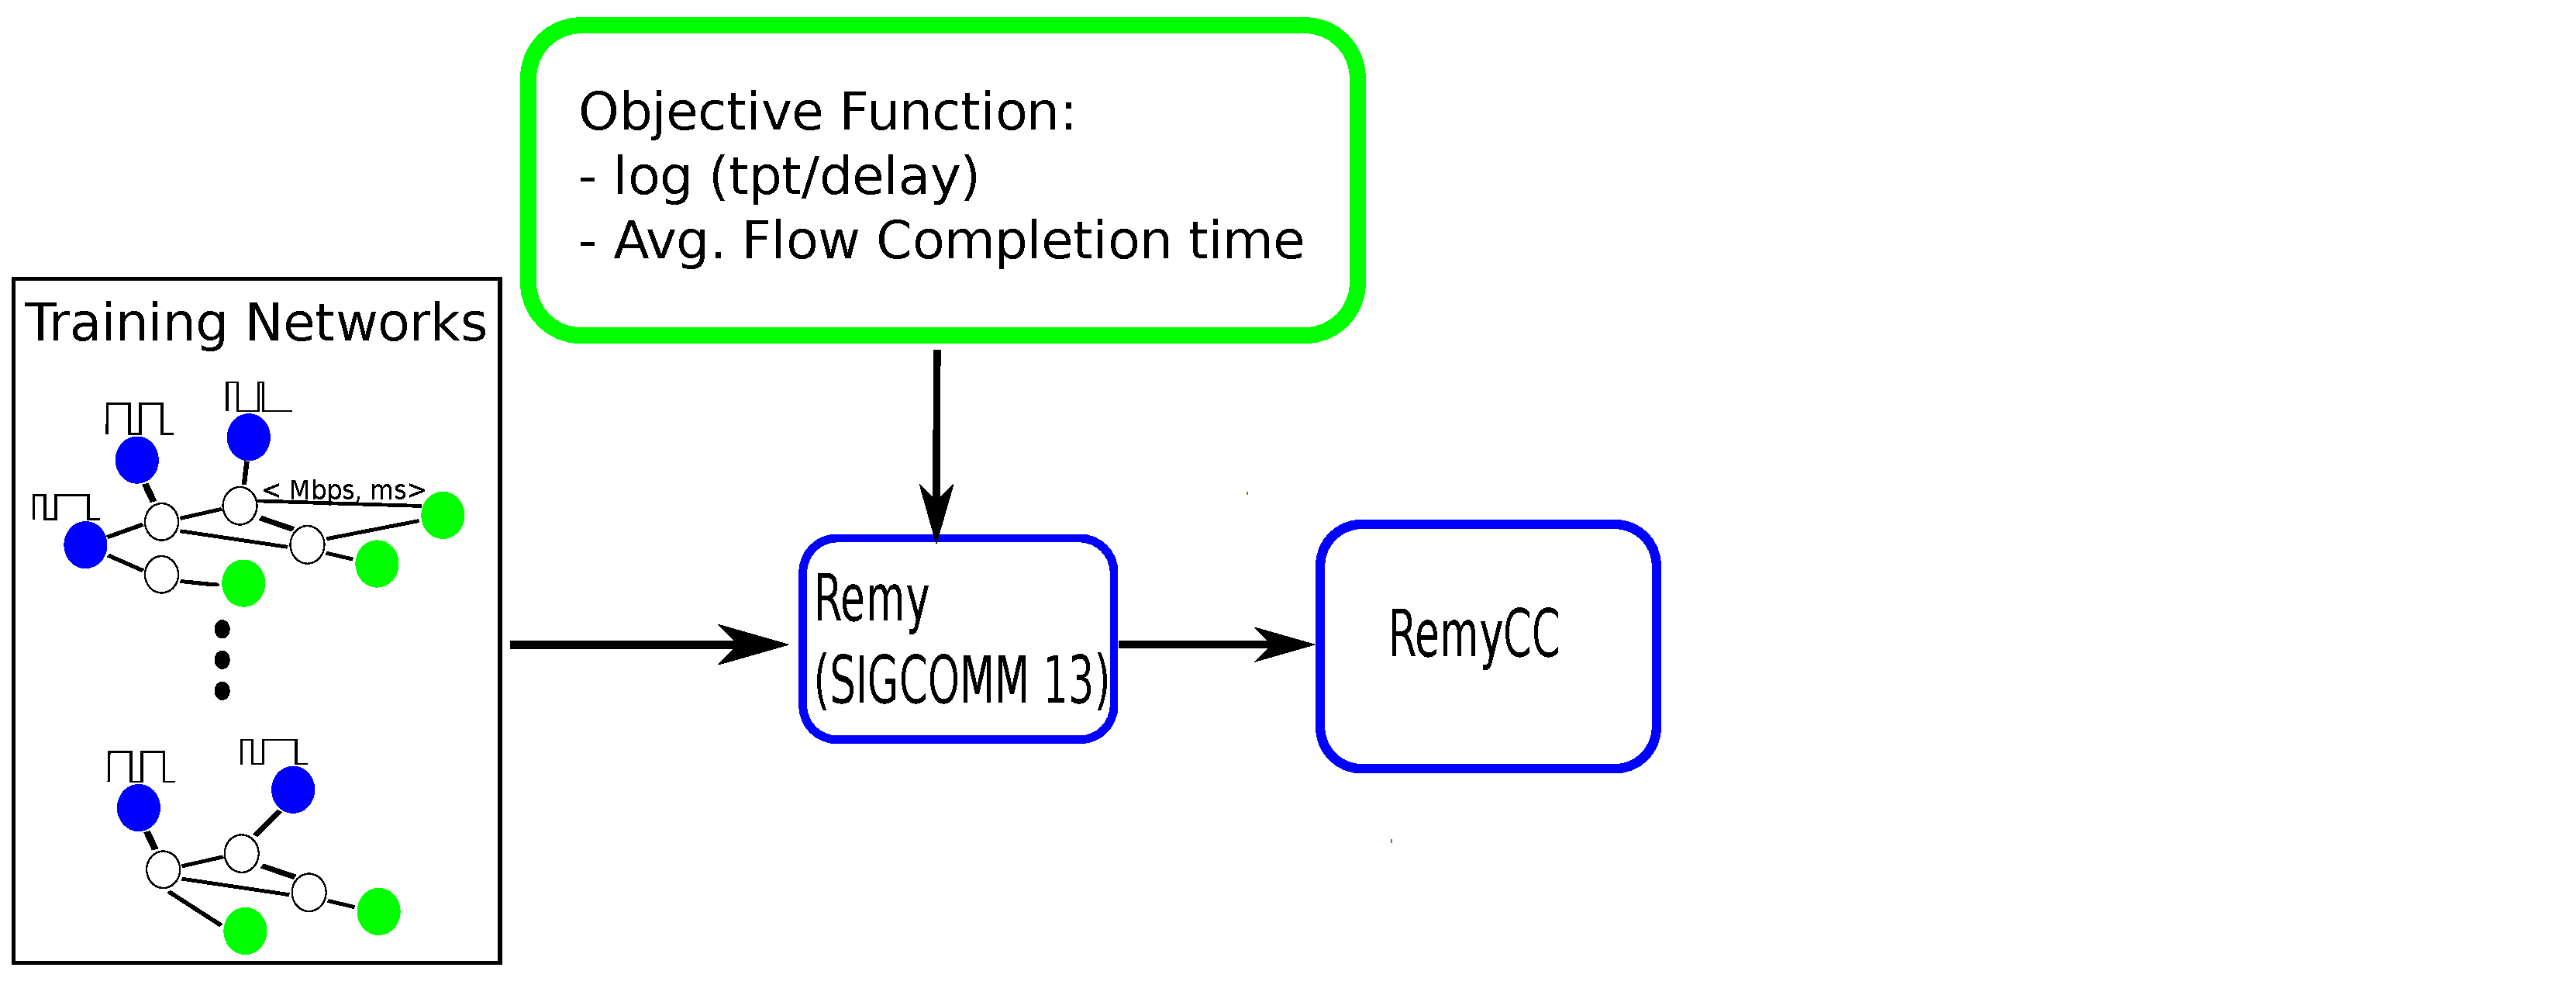
\includegraphics[width=4.5 in]{mechanize-4.pdf}}\only<5>{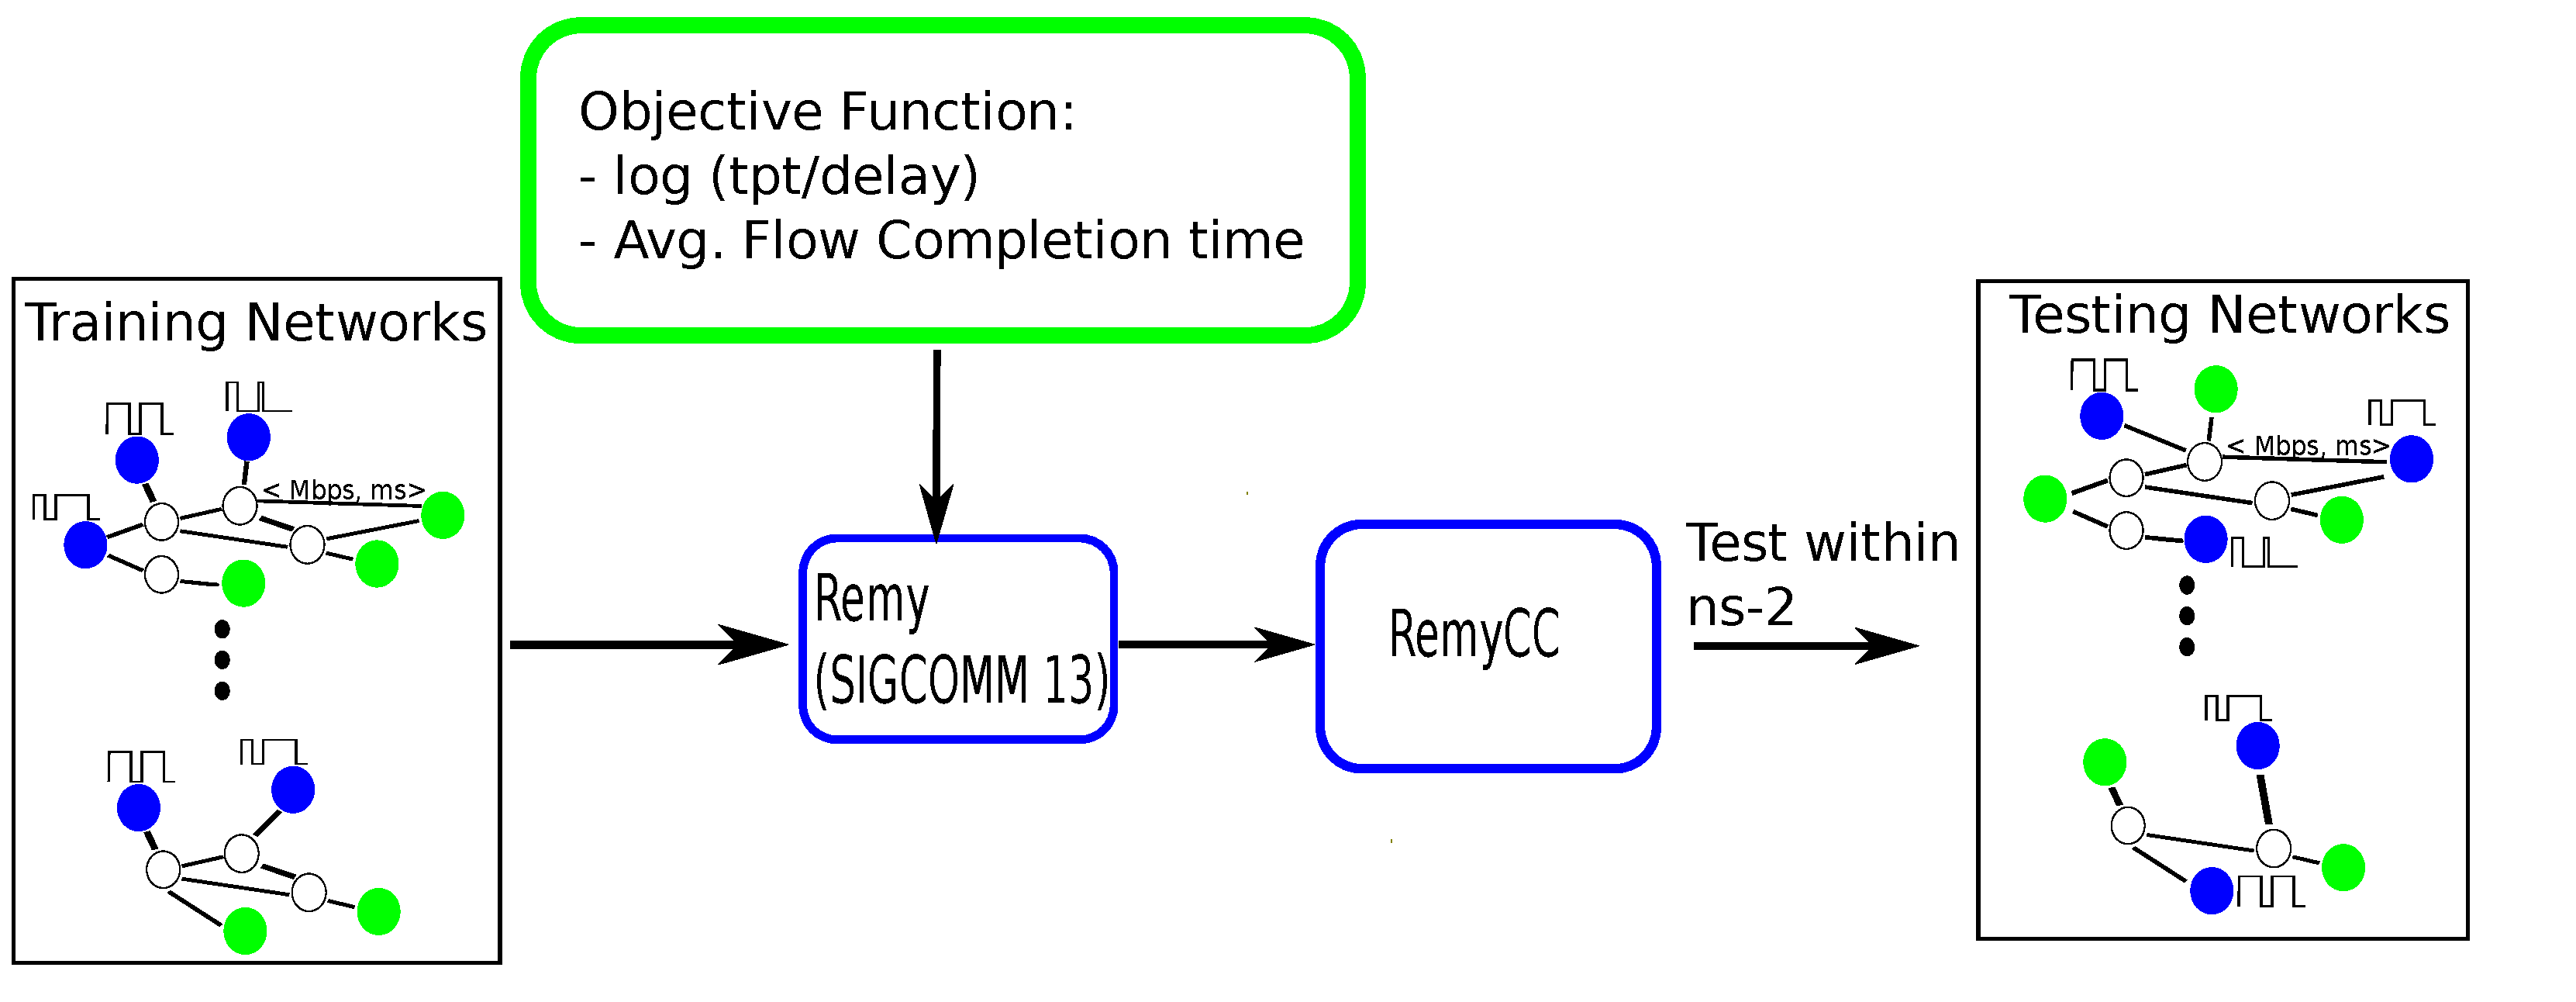
\includegraphics[width=4.5 in]{mechanize-5.pdf}}
\end{frame}

\input optimality

\input linkspeed

\input multiplexing

\input topology 

\input compatibility

\begin{frame}
\frametitle{Caveats}
\begin{itemize}
\item<2-> Remy as a proxy for an optimal learner
\item<3-> Results may change with better learners
\item<4-> Negative results may no longer hold
\end{itemize}
\end{frame}

\begin{frame}
\begin{center}
Learnability in the real world
\end{center}
\end{frame}

% Maybe three separate slides: WANs, datacenters, switch support
\begin{frame}
\frametitle{Protocols for wide-area networks}
\begin{itemize}
\item<1-> Objectives:
\begin{itemize}
\item File-transfer times
\item Page-load times
\item Stall-free video
\end{itemize}
\item<2-> Do we need to optimize for each objective separately?
\end{itemize}
\end{frame}

\begin{frame}
\frametitle{Learning datacenters}
\begin{itemize}
\item<1-> Objective: tail flow-completion time for short flows
\item<2-> Workload varies spatially and temporally
\item<3-> Optimize for each workload separately?
\end{itemize}
\end{frame}

\begin{frame}
\frametitle{Network-assisted congestion control}
\begin{itemize}
\item<1-> No single in-network scheme is best [ref].
\item<2-> Flexible switch architectures (TPP, RMT).
\item<3-> Does switch support for congestion control change any of
our conclusions?
\end{itemize}
\end{frame}

\begin{frame}
\frametitle{The learnability of congestion control}
\noindent
\begin{itemize}
\item<2-> \textcolor{darkgreen}{Can tolerate mismatched link-rate assumptions}
\item<3-> \textcolor{red}{Need precision about the number of senders}
\item<4-> \textcolor{darkgreen}{Can tolerate mismatch in the \# of bottlenecks}
\item<5-> \textcolor{red}{TCP compatibility is a double-edged sword}
\item<6-> http://web.mit.edu/remy/learnability
\end{itemize}
\end{frame}

\end{Large}

\begin{frame}[noframenumbering]
\frametitle{Backup slides}
\end{frame}
\input remy
\input diversity
\end{document}
